\documentclass[a4paper,14pt]{extarticle}

\usepackage[T2A]{fontenc}
\usepackage[utf8]{inputenc}
\usepackage[english,russian]{babel}
\usepackage[left=3cm, right=1.5cm, top=2cm, bottom=2cm]{geometry}
\usepackage{setspace}
\onehalfspacing%
\usepackage[center]{titlesec}
\usepackage{indentfirst}
\setlength{\parindent}{20pt}
\usepackage{fancyhdr}
\pagestyle{fancy}
\fancyhf{}
\fancyhead[C]{\thepage}
\renewcommand{\headrulewidth}{0pt}

\usepackage[acronym]{glossaries}

\usepackage{multirow}
\usepackage[hidelinks]{hyperref}

\usepackage{graphicx}
\graphicspath{{images/}}

\usepackage{miller}
\newcommand{\unit}[1]{ \ \text{#1}}
\newcommand{\degree}{^\circ}
\newcommand{\YEu}{${(\text{Y}_{1-x}\text{Eu}_x)}_2\text{O}_3$}
\newcommand{\range}[2]{[#1\div#2]}

\author{Кудрявцев А.Л.}
\title{Разработка прецизионного метода определения параметров элементарной ячейки для монокристального дифрактометра, оснащенного двумерным детектором}

\begin{document}
\maketitle
\newpage
\tableofcontents
\newpage
\section{Введение}
\subsection{Обзор методов}

Были изучены обзорные статьи~\cite{Lider:2020,Galdecka:2006}.
В них производятся обзоры рентгеновских дифракционных методов измерения параметров элементарной ячейки (ПЭЯ).
Среди них выбирался тот, который можно адаптировать под стандартный лабораторный монокристальный дифрактометр.
Такой дифрактометр предполагается оснащенным:
\begin{itemize}
    \item Рентгеновской трубкой с хорошо монохроматизированным и колимированным пучком.
    \item Как минимум моторизированным однокружным гониометром для образца.
    \item Матричным детектором регулируемым углом поворота.
\end{itemize}
Таким образом из всего многообразия методов сразу исключаются интерференционные, полихроматические, а также использующие сильно расходящийся пучок методы. Также исключаются методы, требующие установки дополнительных монохроматоров и колиматоров.
Среди оставшихся можно выделить методы:
\begin{itemize}
    \item Бонда
    \item Обратного рассеяния
    \item Компланарных рефлексов
    \item Реннингера
    \item Эталонов
\end{itemize}
Метод Бонда среди них --- простой, безэталонный, универсальный в реализации, не имеющий строгих требований и дающий при аккуратном проведении эксперимента очень хорошую точность.
Его идея и взята за основу разработанной нами методики.
\subsection{Метод Бонда}
В оригинальном исполнении~\cite{Bond:1960} схема Бонда представляет собой однокристальный спектрометр~\ref{fig:bond}.
В качестве источника используется колимированный монохроматизированный пучок.
Кристалл --- это ориентированная монокристаллическая пластинка, размерами превосходящая первичный пучок.
Детектор используется точечный, с возможностью вращаться вокруг той же оси, что и кристалл.
Само измерение угла дифракции в схеме Бонда выглядит так:
\begin{enumerate}
    \item Выбирается плоскость кристалла, отражение от которой будет измеряться
    \item Детектор устанавливается под углом, чтобы зарегистрировать отражение от плоскости
    \item Измеряется зависимость интенсивности на детекторе от угла поворота $\omega$ кристалла вблизи отражающего положения
    \item Из полученной зависимости определяется угол $\omega_1$ при котором достигается максимум интенсивности на детекторе
    \item Предыдущие три шага повторяются для симметричного положения детектора и определяется второй угол $\omega_2$
    \item Угол дифракции вычисляется как $2\theta=180^\circ-|\omega_1-\omega_2|$
\end{enumerate}
Определение угла $2\theta$ по такой схеме является более точным чем по одиночному отражению, так как вычисляя разницу углов $\omega$ исключаются ошибки связанные с эксцентриситетом, поглощением и нулевым положением угла $\omega$.

Схема Бонда была адаптирована и для изучения малых монокристаллов~\cite{Hubbard:1976,Ponomarev:1969}.
В этом случае уже не исключаются ошибки, связанные с эксцентриситетом образца.
Для их компенсации изначальную методику дополнили измерением углов $\omega$ отражений для фриделевской пары изначальной плоскости.
Таким образом суммарно для измерения одного межплоскостного расстояния нужно снять профили 4 различных рефлексов.

Для трехкружного гониометра используются методики измерения 8 различных рефлексов~\cite{King:1979}.
В такой схеме можно учесть все ошибки, связанные со смещением образца от точки сведения осей гониометра, а также определить нулевые положения гониометра.

Ключевой особенностью современных монокристальных дифрактометров является использование двумерных детекторов, которое, с одной стороны уменьшает время сбора данных для рентгеноструктурного анализа (РСтА), а с другой негативно влияет на их качество~\cite{Dudka:2017}.

Методика точного измерения угла дифракции при использовании двумерного детектора по аналогии с оригинальной схемой оказывается во многом не удобной.
В том числе необходимость ручного суммирования сигнала и обработки большого числа снимков.
В качестве альтернативы был выбран метод, использовавшийся в~\cite{Serebrennikova:2021}.

В этом методе снимается не зависимость интенсивности от угла поворота кристалла $I(\omega)$, а двумерный профиль интенсивности при полном равномерном повороте кристалла вокруг оси $\omega$ через отражающее положение.
В таком случае, вид зависимости интенсивности от координат детектора в основном определяется спектром первичного пучка.
Зная его можно довольно точно определять положения дифракционных пиков на детекторе, из которых в дальнейшем можно определить и углы дифракции.
\section{Экспериментальная часть}
\subsection{Описание установки}
Рентгенографические эксперименты проводились на монокристальном дифрактометре Bruker D8 Venture.
\begin{itemize}
    \item Микрофокусная трубка Incoatec $I \mu S \ 3.0$
    \begin{itemize}
        \item $\text{Cu} K\alpha$ и $\text{Mo} K\alpha$ излучение
        \item Монохроматизация и фокусировка с помощью многослойных зеркал Монтеля
        \begin{itemize}
            \item Диаметр пучка $110\unit{мкм}$
            \item Расходимость пучка $0.3\degree$
        \end{itemize}
    \end{itemize}
    \item Двумерный детектором PHOTON III
    \begin{itemize}
        \item Разрешение $768 \times 1024$ пикселей
        \item Размер пикселя $135 \times 135\unit{мкм}^2$
        \item Ручная установка расстояния до образца
    \end{itemize}
    \item Трехкружный гониометр FIXED-CHI
    \begin{itemize}
        \item Угол $\chi$ фиксирован и равен $54.7112\degree$
        \item Паспортная воспроизводимость установки углов $0.0001\degree$
        \item Паспортная точность установки углов не указана, но согласно результатам измерения эталонного образца на порошковом дифрактометре Bruker D8 Advance, оснащенном аналогичным гониометром, она не хуже $0.005\degree$
    \end{itemize}
    \item Температурная приставка Oxford Cryostream 800Plus
    \begin{itemize}
            \item Стабильность поддержания температуры $0.2\unit{К}$
    \end{itemize}
    \item Управление прибором средствами программного пакета APEX3~\cite{Bruker:2019}.
\end{itemize}
Необходимо отметить, что из-за расположения трубок область доступных углов для детектора оказывается ограниченной.
Для использовавшегося расстояния от образца до детектора около $130\unit{мм}$, угол $2\theta_D$ не мог превосходить примерно $100\degree$.

\begin{figure}[ht!]
    \centering
    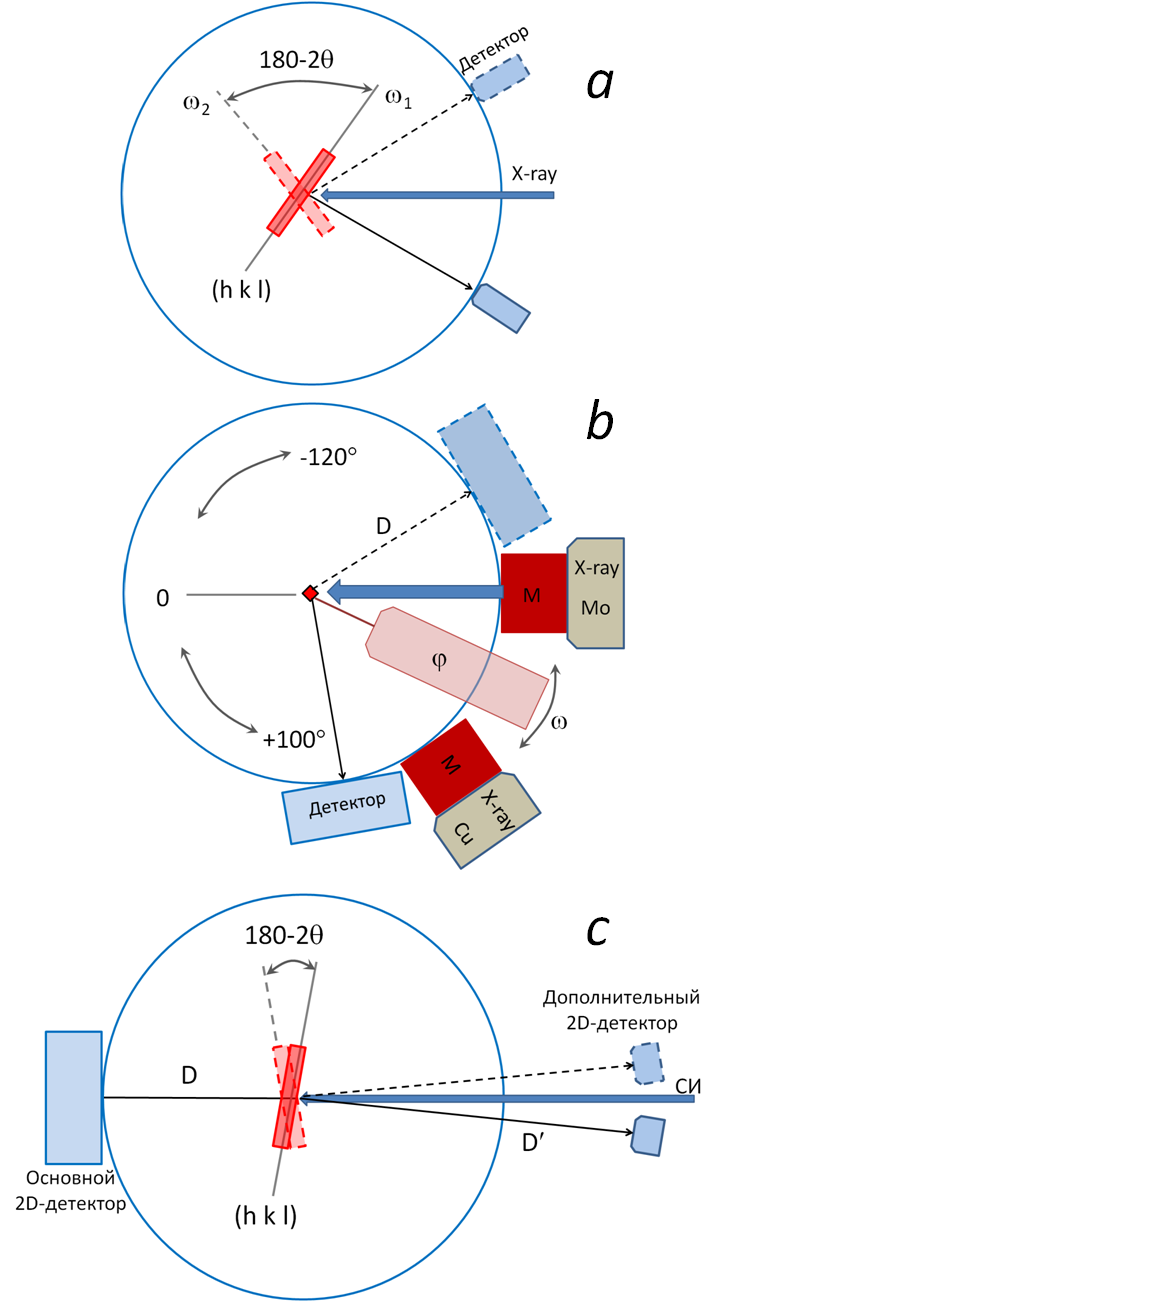
\includegraphics[width=0.8\textwidth]{bond.png}
    \caption{Варианты реализации схемы Бонда: $a$ --- классическая схема с использованием ориентированной кристаллической пластинки и однокружного гониометра. При съемке неподвижный точечный детектор регистрирует изменение интенсивности при изменении угла $\omega$ в режиме $I(\omega)$; $b$ –-- схема, реализованная в настоящей работе. Кристалл c размерами меньше диаметра первичного пучка выводится в отражающее положение путем установки определенных углов $\varphi$ и $\omega$. Неподвижный $2D$--детектор регистрирует суммарную дифракционную картину при изменении угла $\omega$ в интервале $\pm 2\degree$. Пунктирная дуга показывает область возможного размещения детектора, сплошная – держателя гониометрической головки.}
    \label{fig:bond}
\end{figure}

Значения характеристических длин волн, использованных в этой работе приведены в таблице~\ref{tab:wavelengths}.
\begin{table}[ht!]
    \centering
    \begin{tabular}{ |c|c|c| }  
        \hline
        Анод & $K\alpha_1,\unit{\AA}$ & $K\alpha_2,\unit{\AA}$ \\
        \hline
        Cu & 1.54059290 (50) & 1.54442740 (50) \\
        Mo & 0.70931715 (41) & 0.713607 (12) \\
        \hline
    \end{tabular}
    \label{tab:wavelengths}
    \caption{Использовавшиеся значения характеристических длин волн}
\end{table}
\subsection{Исследуемые образцы}
Для определения точности методики были использованы эталонные монокристаллы Si и Ge.

Изученный монокристалл Si имел линейные размеры примерно 50~мкм.
Он является осколком кристалла, который ранее был исследован на однокристальном спектрометре~\cite{Lisoivan:1982}.
Значение $a = 5.430933(12)\unit{\AA}$ там было получено с использованием значение длины волны $\lambda \text{Cu} K \alpha_1 = 1.540562\unit{\AA}$.
При пересчете на более точное значение из~\ref{tab:wavelengths}, эталонное значение ПЭЯ для Si
\[ a_\text{Si} = 5.431042 (12)\unit{\AA}. \]

Изученный монокристалл Ge также был размером около 50~мкм.
ПЭЯ Ge уточняли несколько раз методами однокристального спектрометра, многократных отражений и многолучевой дифракции: сводка данных приведена в~\cite{Lisoivan:1982}.
Значения ПЭЯ Ge лежат в интервале от $5.65776 (2)\unit{\AA}$ до $5.657837 (15)\unit{\AA}$, среднее значение $5.65779$ наиболее близко к $5.657772 (10)\unit{\AA}$~\cite{Cooper:1962}.
Пересчет с использованием более точного значения длины волны приводит к
\[ a_\text{Ge} = 5.657885 (10)\unit{\AA} \]

Также с целью определения однородности продукта синтеза был изучен твердый раствор \YEu.
Для этого было отобрано 5 различных монокристаллов.
Для каждого из них был проведен РСтА и измерение ПЭЯ по разработанной методике.
\subsection{Описание методики}
Первое описание методики дано в статье~\cite{Kudryavtsev:2024:YEu}.
Общая схема проведения измерений выглядит примерно так:
\begin{enumerate}
    \item Отбор монокристалла
    \item Предварительная съемка
    \item Выбор рефлекса
    \item Съемка рефлекса
    \item Обработка профилей
    \item Расчет межплоскостного расстояния
\end{enumerate}
\subsubsection{Отбор монокристалла}
Отбор монокристалла проводится так же, как и для РСтА.
Монокристалл выбирается так, чтобы не превосходить размера первичного пучка.
В нашем случае оптимальный размер равен приблизительно 50~мкм.
\subsubsection{Предварительная съемка}
Предварительная съемка проводится с целью определения ориентации кристалла, его дифракционного класса и получения данных об интенсивности рефлексов.

Сама съемка состоит серии полных сканирований при вращении вокруг оси $\varphi$ с шагом $0.5\degree$ для при фиксированном угле $\omega$.
Три таких сканирования выполняются при углах детектора $2\theta_D = -45\degree, 0\degree, 45\degree$ при фиксированном расстоянии до образца $D \approx 70\unit{мм}$.

Обработка снимков и получение ориентации производится в программе APEX3.
На выходе программы получается файл формата p4p, где информация об ориентации кристалла содержится в виде UB матрицы~\cite{Busing:1967}.
\subsubsection{Выбор рефлекса}
Выбор рефлекса для съемки происходит так, чтобы погрешность измерений была минимальной.
Основными критериями в таком случае оказываются наибольшие угол $2\theta$ и интенсивность рефлекса.
При этом необходимо учитывать геометрию установки, так как не все рефлексы оказывается возможно вывести в отражающее положение для двух симметричных положений в экваториальной плоскости.

Средствами программы APEX3 производить такой перебор рефлексов неэффективно и крайне проблематично, так как программа рассчитывает для одного рефлекса максимум только одну пару углов $(\varphi, \omega)$ из двух возможных в общем случае.
Поэтому была специально написана программа~\cite{Kudryavtsev:2024:eccentr} для перебора всех рефлексов, расчета для них углов гониометра и отбора случаев когда в оказывается возможным вывести рефлекс в два симметричных положения, а также когда доступна для выведения и его фриделевская пара.

Программа позволяет находить среди множества плоскостей, связанных симметрией такие, которые можно вывести в отражающее положение хотя бы при одном (из двух симметричных) положений детектора.
Для этого используется информация о текущей ориентации кристалла на гониометре, т.е. p4p-файл, в котором находится матрица ориентации UB и предварительные значения ПЭЯ.
Используя известную длину волны, размеры пикселя, расстояние до детектора, и другие неизменные параметры прибора, программа вычисляет углы гониометра $(\varphi, \omega)$, необходимые для выведения каждой плоскости в отражающее положение на экваториальную плоскость.
В каждом случае проверяются геометрические ограничения прибора.
Полученная информация для всех подходящих рефлексов собирается в таблицу Excel, ее можно проанализировать и провести отбор.
\subsubsection{Съемка рефлекса}
Съемка рефлекса представляет собой сканирование при вращении вокруг оси $\omega$ в диапазоне $\pm 2\degree$ относительно рассчитанного значения $\omega$ для отражающего положения.
Время съемки выставлялось таким, чтобы максимум на профиле пика составлял не менее 10000~имп.

В программе APEX3 невозможно выставить время съемки больше 10~мин., поэтому для достижения последнего условия производились несколько одинаковых съемок по 10~мин. пока не будет достигнута требуемая интенсивность.
\subsubsection{Обработка профилей}
Обработка профилей состоит из нескольких этапов, по завершению которых можно рассчитать межплоскостное расстояние.
Реализована она была тоже в виде программы~\cite{Kudryavtsev:2024:eccentr}.

На входе она использует p4p-файл и информацию о примерном положении центра детектора (результат юстировки, прямое определение, калибровка).
Из экспериментального фрейма вырезается центральная область $X = \pm 30\unit{пикс.}, Y = \pm 15\unit{пикс.}$, в которой, исходя из условия $2\theta_D \approx 2\theta$, должен находиться искомый рефлекс.
Медианное значение интенсивности принимается за начальное значение фона.
Пиксели с интенсивностью больше заранее заданной принимаются за "горячие пиксели" и их значения приравниваются среднему значению по 8 соседним пикселям.
После учета горячих пикселей максимум интенсивности в выбранной области назначается примерным положением $K\alpha_1$--составляющей.
Далее, исходя из значений $D$ и $2\theta$ рассчитывается положение $K\alpha_1$--составляющей и обе точки смещаются так, чтобы теоретическое положение $K\alpha_1$ совпадало с координатами найденного максимума интенсивности.
Аппроксимация дублета проводится двумя независимыми  функциями 2D-Gauss, т.е. без закрепления междублетного расстояния и соотношения интенсивностей составляющих $2/1$.
Направлениями главных осей берутся вдоль координат детектора $X$ и $Y$ детектора.
В наших экспериментах именно функция 2D-Gauss наиболее хорошо описывала форму пика при минимальном числе уточняемых параметров: координаты максимума, полуширины (ширина на половине высоты, FWHM) в направлениях $X$ и $Y$, и интегральная интенсивность.
\subsubsection{Рассчет межплоскостного расстояния}
Для достаточно малой разницы координат рефлексов искомый угол дифракции можно рассчитать по формуле
\begin{equation} \label{eq:bond2}
    2\theta = 2\theta_D - \frac{\gamma}{2} (X_{+} - X_{-}),
\end{equation}
где $\gamma$ --- угловой размер пикселя в точке детектирования рефлекса, $X_{-}, X_{+}$ --- координаты рефлексов при отрицательном и положительном углах детектора.
В формуле $2\theta_D$ предполагается положительным.
Знак перед разницей координат рефлексов зависит от направления координаты $X$ детектора и направлением положительного вращения детектора вокруг оси $2\theta_D$.
Если они направлены в разные стороны, то знак ``$-$'', если в одну, то ``$+$''.
В нашей установке направления выбраны так, что перед разницей должен быть ``$-$''.
\subsection{Учет эксцентриситета}
Дополнительная съемка фриделевских пар позволяет учитывать эффект смещения кристалла при вращении вокруг оси $\omega$.
Так как рефлекс при съемке выводится в экваториальную плоскость, то угол $\omega$ для фриделевской пары изначального рефлекса отличается на $180\degree$.
Так как при повороте на $180\degree$ положение кристалла как бы отражается относительно оси $\omega$, то среднее значение координат рефлексов в этих двух положения будет соответствовать положению кристалла ровно на оси $\omega$~\ref{fig:eccentr}.

\begin{figure}[ht!]
    \centering
    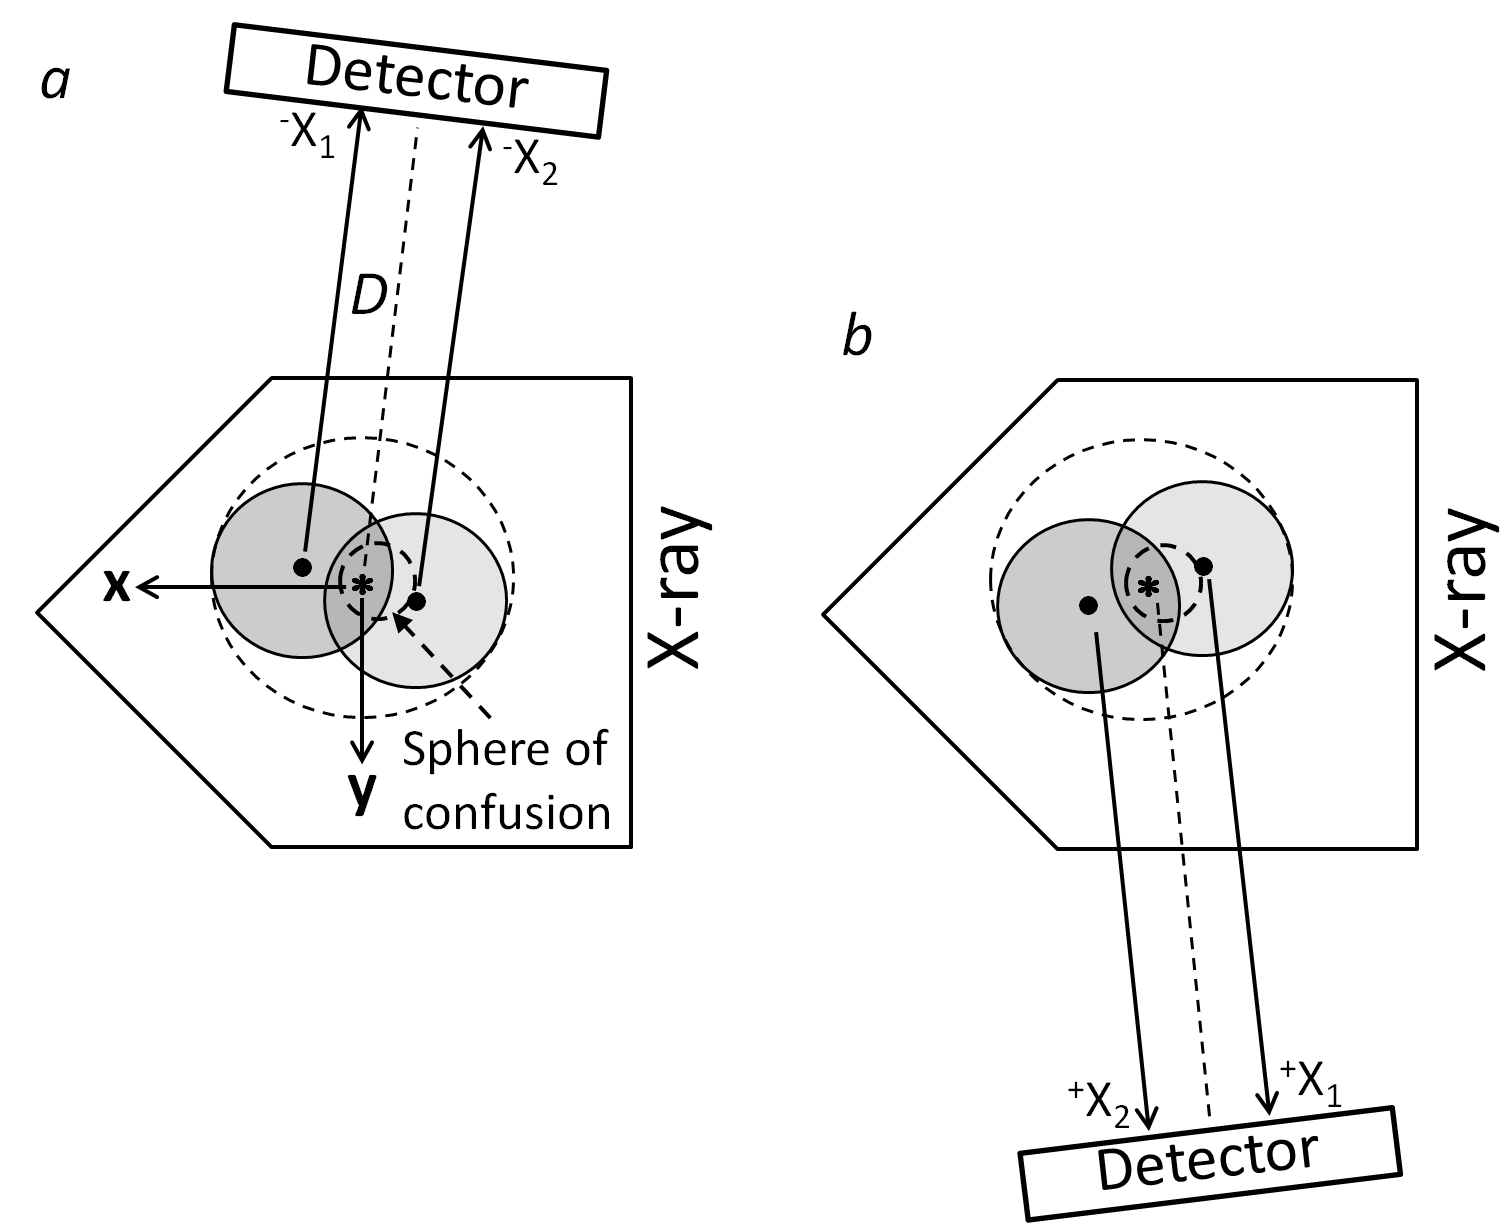
\includegraphics[width=0.8\textwidth]{eccentr.png}
    \caption{Схемы эксперимента для учета эксцентриситета образца, связанного с поворотом вокруг оси $\omega$ (ось $\omega$ идет перпендикулярно плоскости чертежа, выход показан звездочкой). $a$ --- показаны два положения образца (условные центры обозначены жирными точками), при которых проводятся съемки рефлексов и определяются положения максимумов –-- $X_1$ и $X_2$. Окружность меньшего диаметра соответствует сфере сведения, большая окружность (выделена пунктиром) ограничивает область расположения образца. Показана система координат: направление $x$ проходит через ось $\omega$ в направлении первичного пучка (условно показано, что в общем случае $x$ не совпадает с максимумом первичного пучка); $y$ --– направление перпендикулярное $x$ и лежащее в экваториальной плоскости. Направление $z$ совпадает с осью $\omega$. $b$ –-- схема для симметричного положения детектора.}
    \label{fig:eccentr}
\end{figure}

Таким образом измерение фриделевской пары позволяет использовать уточненное значение координат рефлекса
\[X_{true} = \frac{1}{2}(X + X_{frid})\]
где $X, X_{frid}$ --- координаты обычного рефлекса и его фриделевской пары соответственно.
Подставляя это в формулу~\ref{eq:bond2} получим
\begin{equation} \label{eq:bond4}
    2\theta = 2\theta_D - \frac{\gamma}{4} (X_{+} + X_{+frid} - X_{-} - X_{-frid}).
\end{equation}
\subsection{Расчет углового размера пикселя}
Зная линейные размеры пикселя $P$ и расстояние до центра детектора $D$ можно с хорошей точностью рассчитать угловой размер пикселя как
\begin{equation} \label{eq:gamma_simple}
    \gamma = \frac{P}{D}.
\end{equation}
В нашем случае $P = 135\unit{мкм}$, а расстояние $D$, указываемое прибором $D = 128.53\unit{мм}$.

Однако значение $D$, которое показывает прибор, всегда можно поставить под сомнение.
Правильнее провести калибровку положения детектора, например, согласно методике~\cite{Panchenko:2023}.
Для этого съемка эталонного монокристалла Si была проведена путем $\omega$--сканирования интервалов $10\degree$ в области углов $200\degree$ при пяти положениях кристалла по углу $\varphi$ (шаг $10\degree$).
Обработка полученных фреймов проведена по программе SearchXY~\cite{Panchenko:2023}.
В результате получено значение $D = 128.21\unit{мм}$.
Развороты детектора в наших экспериментах можно не учитывать из-за их малости и так как регистрация рефлексов проводится центральной областью детектора.

Полная калибровка занимает достаточно много времени и не всегда целесообразна.
Другой подход к определению $\gamma$ основан на съемке одного и того же рефлекса при двух угловых положениях детектора.
Так, рефлекс $\hkl(11 3 1)$ эталонного монокристалла Si был отснят при $2\theta_D = 96.4\degree, 97.0\degree$.
Смещение рефлекса $\Delta X$ позволяет провести вычисление $\gamma$ по формуле
\begin{equation} \label{eq:gamma_delta}
    \gamma = \frac{\Delta 2\theta_D}{\Delta X}
\end{equation}

Отметим, что такой подход позволяет проводить измерения при минимальных отклонениях рефлекса от центра детектора.
Полученное значение идеально совпадает с результатом, полученным по результатам полной калибровки.
Итоговое значение, использовавшееся далее
\[ \gamma = 0.06033\degree \]
\section{Обсуждение результатов}
\subsection{Изучение Si}
Измерение проводилось в нескольких переустановках образца и разных расстояниях $D$ и углах $2\theta_D$.
Также для оценки возможности использования рефлексов отстоящих от центра детектора съемка фриделевской пары $\hkl(-9 7 1)/\hkl(9 -7 -1)$ была проведена при положении детектора $2\theta_D = \pm 97.5\degree$, что является крайним положением для $D = 128.5\unit{мм}$, которое отличается от идеального почти на $0.8\degree$.
Исследование фриделевской пары $\hkl(3 -3 1)/\hkl(-3 3 -11)$ показало разницу координат $Y$ всего 4~пикс.
Среднее значение отклонение экспериментально полученных значений $2\theta$ от эталонных составило $0.0003\degree$, а среднее значение ПЭЯ отличается от эталонного на $0.0001\unit{\AA}$.
Относительная погрешность определения $d$ и ПЭЯ составила $5 \times 10^{-5}$.
\subsection{Изучение Ge}
На монокристалле Ge проводили контроль воспроизводимости установки образца и детектора.
Для этого было выполнено несколько переустановок образца, в том числе с коррекцией ориентации кристалла, изменением $D$ и угла $2\theta_D$.
При $D = 138.6\unit{мм}$ изучены рефлексы $\hkl(5 -11 -1)$ и $\hkl(1 -11 -5)$ с существенно отличными углами выведения в отражающее положение $(\varphi, \omega)$.
Для оценки возможности использования рефлексов, значительно отстоящих от центра детектора, съемка рефлекса $\hkl(7 -7 -7)$ была проведена при двух разных значениях $2\theta_D$.
Причем положение $\pm 99.9\degree$ отличалось от идеального почти на $1\degree$.
Исследование фриделевской пары $\hkl(3 -3 11)/\hkl(-3 3 -11)$ показало хороший уровень точности выведения рефлексов на экваториальную плоскость: разница координат $Y$ не превысила $\approx 7\unit{пикс.}$, что составляет $\approx 0.4\degree$.
В результате обработки профилей рефлексов были получены координаты максимумов и по формуле~\ref{eq:bond2} определены углы $2\theta$, а из них рассчитаны значения $d$ и ПЭЯ.
Среднее отклонение полученных значений $2\theta$ от теоретических составило $0.004\degree$, что соответствует точности гониометра.
Если ориентироваться на полученную величину, то относительная погрешность определения межплоскостного расстояния $\Delta d / d = 6 \times 10^{-5}$.
Таким образом, абсолютную погрешность определения ПЭЯ для Ge можно оценить как $0.0003\unit{\AA}$.
Среднее значение $a_\text{Ge} = 5.6579\unit{\AA}$ отличается от эталонного значения меньше, всего на $0.0001\unit{\AA}$.
\subsection{Изучение \YEu}
При выборе рефлекса, подходящего для уточнения ПЭЯ, мы столкнулись с проблемой оценки его интенсивности из-за хиральности точечной группы симметрии кристалла.
Так, например, теоретические значения структурной амплитуды рефлексов $\hkl(6 8 20)$ и $\hkl(8 6 20)$ соотносятся как 7 к 1.
Естественно, предпочтительно использовать наиболее интенсивное отражение.
Для решение этой проблемы предварительная съемка кристалла была скорректирована --- расстояние $D$ уменьшено до $60\unit{мм}$, а углы $2\theta_D$ увеличены до $\pm 75\degree$.
В результате были построены сечения обратного пространства, захватывающие область углов $2\theta = \range{95\degree}{100\degree}$.
Сопоставление интенсивностей рефлексов с результатами вычислений программы позволило выбрать оптимальные индексы.
По такой схеме было проведено исследование 5 монокристаллов.
Значения ПЭЯ лежат в интервале $\range{10.6902}{10.7045}\unit{\AA}$.
Разница крайних значений составляет $0.0143\unit{\AA}$.
Это значительно превосходит абсолютную погрешность определения ПЭЯ, равную $0.0007\unit{\AA}$.
Таким образом, можно однозначно утверждать, что синтезированный продукт не однороден.

Для оценки соотношения Y/Eu в изученных монокристаллах \YEu~можно использовать правило Вегарда.
Для построения соответствующей прямой были использованы литературные данные~\cite{Swanson:1954,Morris:1984}.

Для проведения РСтА расчет стратегии съемки для накопления полного массива данных производился для каждого кристалла автоматически с учетом его симметрии $(m\overline{3})$ по предварительно определенной матрице ориентации с использованием пакета программ APEX3.
Далее проводили интегрирование экспериментальных интенсивностей и вводили поправки на поглощение.
Структуры решены с помощью программы SHELXT~\cite{Sheldrick:2015:shelxt} и уточнены с SHELXL~\cite{Sheldrick:2015:shelxl} в графическом интерфейсе OLEX2~\cite{Dolomanov:2009}.
Параметры атомных смещений были уточнены в анизотропном приближении.

В результате установлено, что все изученные кристаллы изоструктурны и представляют собой твердые растворы \YEu, причем смешанными оказываются обе позиции металла.
\begin{figure}[ht!]
    \centering
    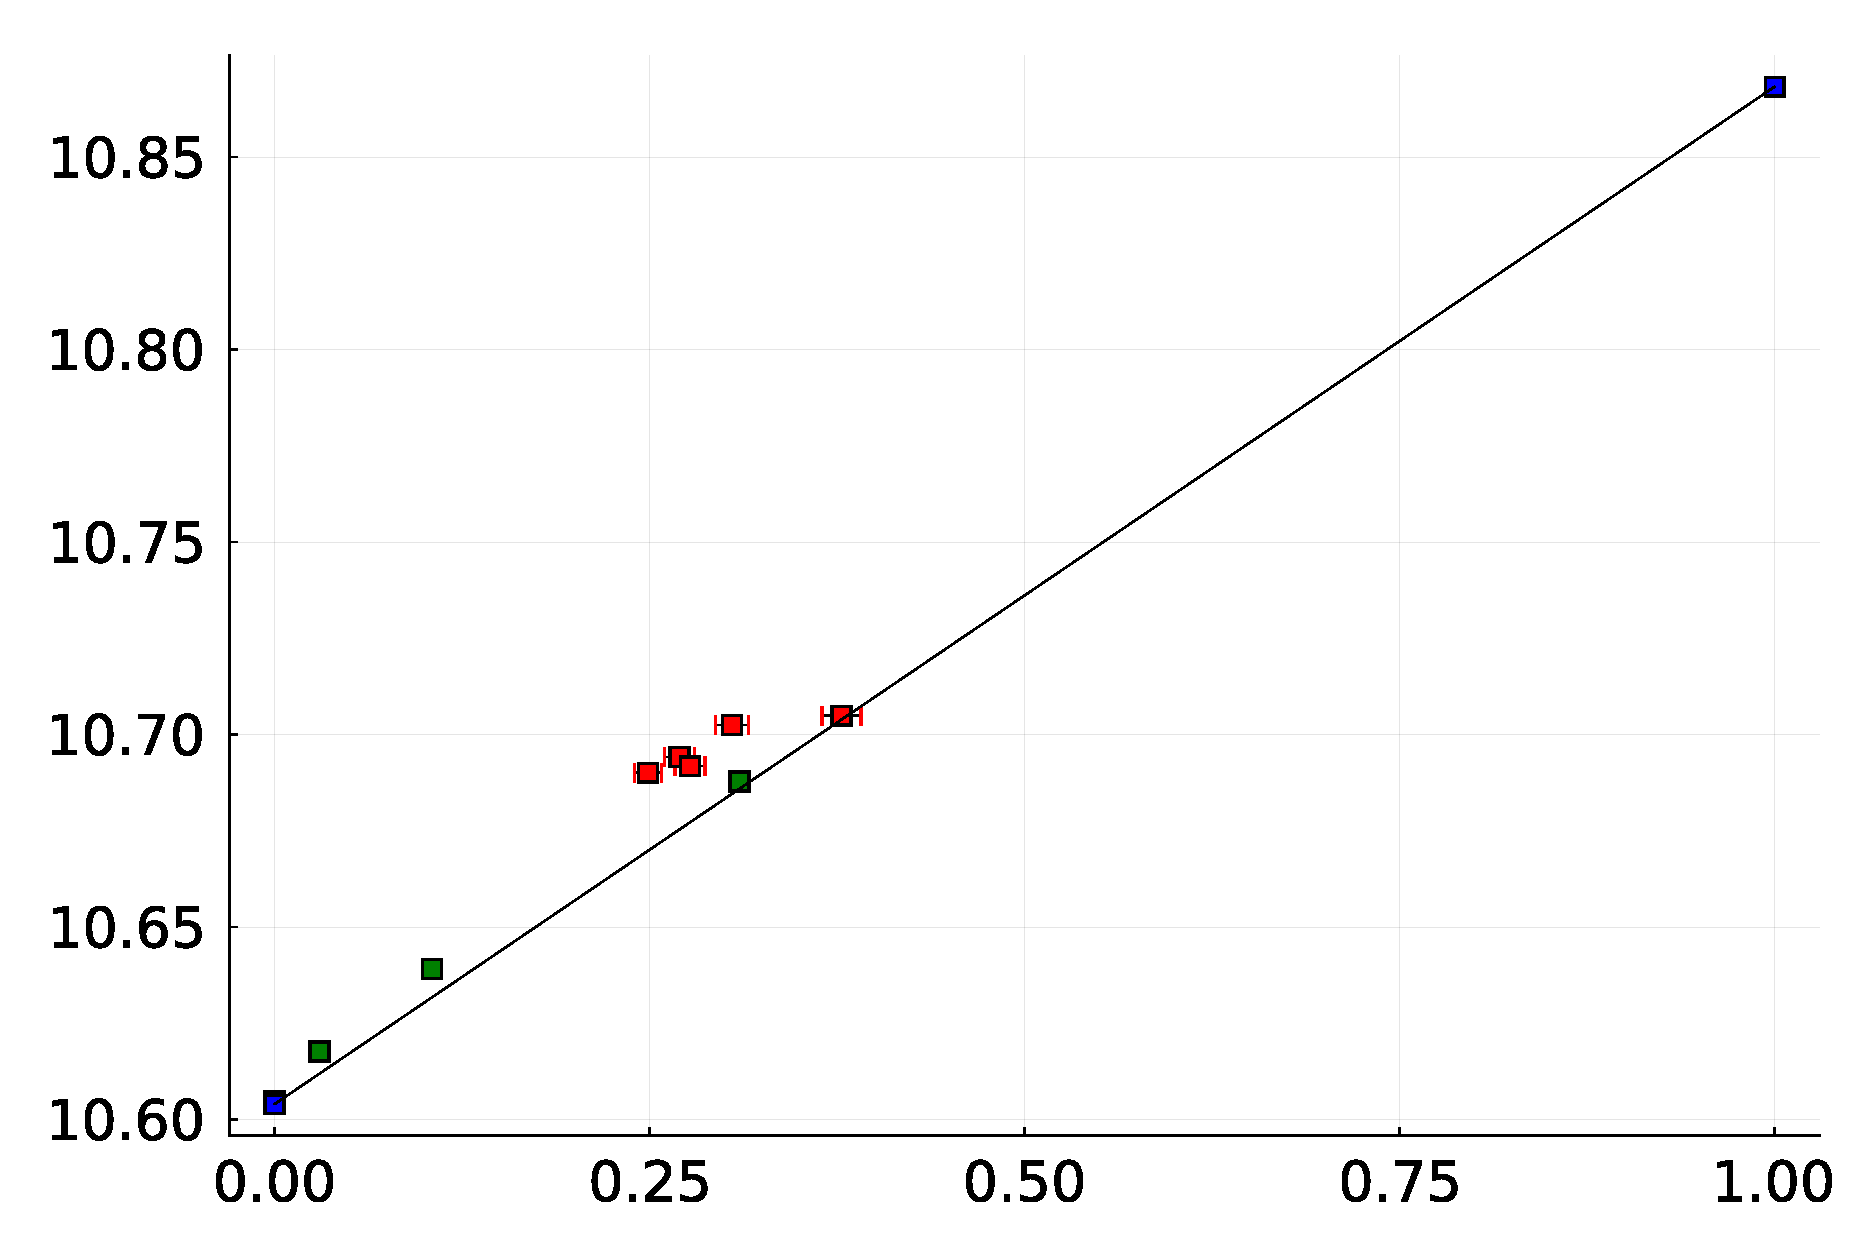
\includegraphics[width=0.8\textwidth]{YEu.pdf}
    \caption{Зависимость ПЭЯ \YEu~от мольной доли $x$.}
    \label{fig:YEu}
\end{figure}

\subsection{Оценка и учет эксцентриситета образца Si}
Несмотря на тщательную центрировку образца, в том числе с контрольными разворотами по оси $\omega$, крайне сложно точно определить его центр, особенно при неопределенной форме кристалла.
Можно ожидать, что при повороте вокруг оси $\omega$ центр образца движется по окружности, а сам образец описывает торообразную поверхность.
Подобную картину можно ожидать и при повороте образца вокруг оси $\varphi$.
Так как для использованного гониометра паспортное значение диаметра сферы сведения осей составляет $7\unit{мкм}$, центр образца при повороте вокруг обеих осей движется по достаточно сложной траектории.

Для оценки смещений центра образца при повороте вокруг оси $\varphi$, среди доступных для измерения рефлексов типов $\hkl{11 3 1}$, $\hkl{9 7 1}$ и $\hkl{9 5 5}$, было выбрано 10 вариантов, у которых значения $\omega$ лежат в интервале $\range{-82\degree}{95\degree}$.
Это примерно соответствует позиции образца при центрировании.
Все съемки проведены при одном положении детектора: $2\theta_D = -96.7\degree$, $D = 128.53\unit{мм}$.

Для оценки эксцентриситета при повороте вокруг оси $\omega$, были отобраны случаи, когда значения $\varphi$ лежат в интервале $\range{283.6\degree}{300.7\degree}$.
При этом соответствующие им углы $\omega$ лежат в интервале $\range{63.3\degree}{296.5\degree}$.
Область $\pm 60\degree$ недоступна из-за геометрических ограничений гониометра.
Графики зависимости координат от углов поворота представлены на графике~\ref{fig:eccentrSi}.

\begin{figure}[ht!]
    \centering
    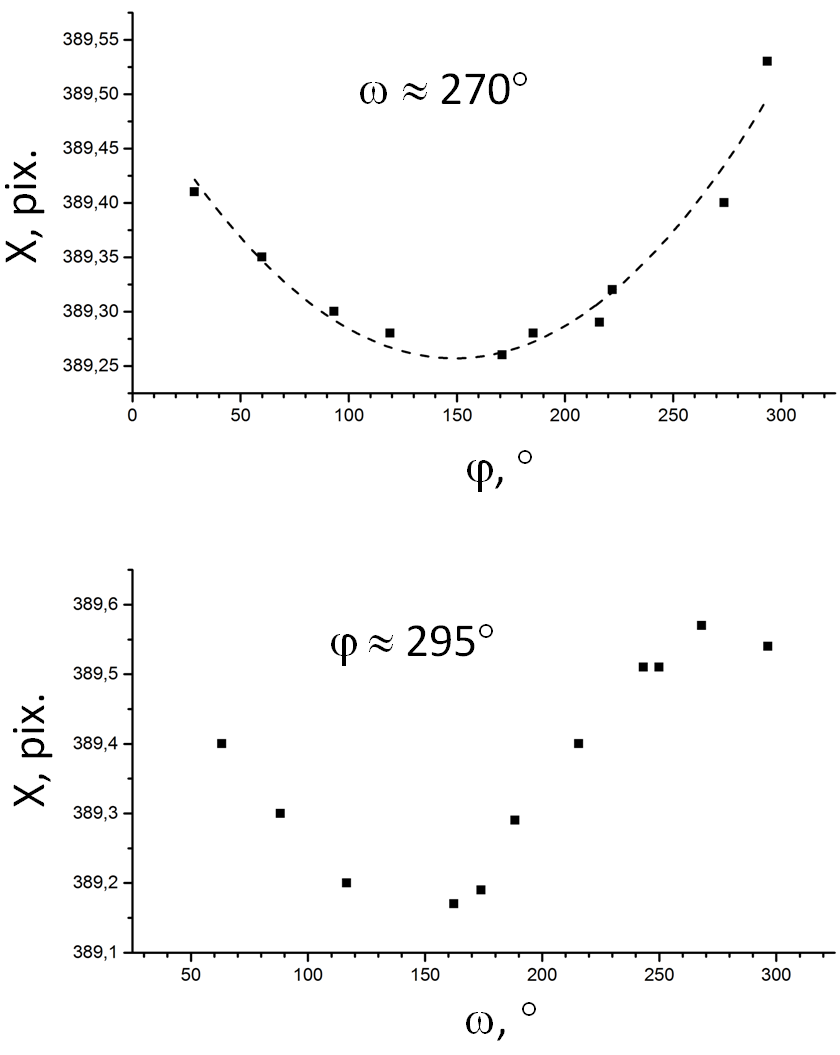
\includegraphics[width=0.8\textwidth]{eccentrSi.png}
    \caption{Смещение максимумов дифракционных отражений $\hkl(11 3 1)$, $\hkl(9 7 1)$ и $\hkl(9 5 5)$ по оси $X$ детектора из-за эксцентриситета образца: $a$ --– зависимость координаты $X$ от угла $\varphi$ (значения углов $\omega \approx 270\degree$); $b$ --- зависимость координаты $X$ от угла $\omega$ (значения углов $\varphi$ лежат в интервале от $\range{283.6\degree}{300.7\degree}$).}
    \label{fig:eccentrSi}
\end{figure}

Таким образом, проведенные два эксперимента показали одинаковую картину для эксцентриситетов, связанных с поворотами образца вокруг осей $\varphi$ и $\omega$.
При измерении ПЭЯ наиболее разумно исключить влияние именно последнего, тогда далее можно использовать подход, описанный выше~\cite{Ponomarev:1969}.

Среди всех вариантов рефлексов были выделены 5 фриделевских пар.
\subsection{Учет эксцентриситета для Si}
При произвольном выборе рефлексов расчет по~\ref{eq:bond2} приводит к значениям угла $2\theta$ в интервале $\range{96.722\degree}{96.747\degree}$.
Учет эксцентриситета по формуле~\ref{eq:bond4} уменьшает интервал значений до $\range{96.730\degree}{96.736\degree}$, а отклонения от теоретического значения не превышают $0.004\degree$.
Использование рефлексов с близкими значениями $\varphi = 66.31\degree, \, 59.35\degree$ позволяет пренебречь эксцентриситетом, связанным с поворотам вокруг оси $\varphi$.
Конечные результаты уточнения представлены в таблице~\ref{tab:Si:eccentr}.
\begin{table}[ht!]
    \centering
    \begin{tabular}{ |c|c| }
        \hline
        $2\theta$ & $96.732\degree$ \\
        $d$ & $0.47452 (3)\unit{\AA}$ \\
        $\Delta d / d$ & $6.2 \times 10^{-5}$ \\
        $a$ & $5.4311 (3)\unit{\AA}$ \\
        \hline
    \end{tabular}
    \caption{Результаты измерений ПЭЯ Si с учетом эксцентриситета.}
    \label{tab:Si:eccentr}
\end{table}

Можно отметить, что полученное значение ПЭЯ отклоняется от эталонного на $0.00006\unit{\AA}$.
Т. е. относительная разница составляет $1\times 10^{-5}$.
Еще раз подчеркнем, что результат получен лишь при частичном учете эксцентриситета, связанного с поворотом кристалла вокруг оси $\varphi$.
Чтобы полностью исключить такое влияние можно вывести одно из кристаллографических направлений вдоль оси $\omega$.
Тогда измерения можно проводить на рефлексах типа $hk0$.
При использовании трехкружного гониометра для образца такая проблема не возникает.
В нашем случае угол $\chi$ --- фиксирован, а штатные гониометрические головки предполагают только линейные смещения образца.
\subsection{Учет эксцентриситета для Ge}
Для устранения эксцентриситета, связанного с поворотом кристалла вокруг оси $\varphi$, монокристалл Ge был смонтирован на оригинальной гониометрической головке, имеющей возможность поворота образца вокруг одной оси на $\pm 10\degree$ (далее гониометрическая $\chi$--головка).
После определения ориентации кристалла были рассчитаны углы для выведения кристаллографического направления вдоль оси $\omega$. Алгоритм этого процесса описан в~\cite{Kudryavtsev:2024:eccentr}.

Расчеты для монокристалла Ge показали, что вдоль оси $\omega$ можно вывести направление $b$, так как для него значения угла $\chi = 2.2\degree$.
После поворота, исследование по нашей методике было проведено по рефлексам типа $\hkl{10 0 6}$.
Им соответствовало значение угла $2\theta = 93.943\degree$.
Все рефлексы регистрировались при одинаковых значениях угла $\varphi = -179.06\degree$.
Геометрические ограничения позволили отснять при $2\theta_D = \pm 93.9\degree$ только 12 из 16 теоретически возможных рефлексов.
При произвольных сочетаниях рефлексов значения $2\theta$, вычисленные по~\ref{eq:bond2} лежат в интервале $\range{93.935\degree}{93.958\degree}$.
Максимальные отклонения от теоретического значения достигают $0.015\degree$.
При использовании формулы~\ref{eq:bond4} углы $2\theta$ укладываются в интервал $\range{93.943\degree}{93.945\degree}$.
Отклонения от теоретического значения в таком случае не превышают $0.001\degree$.
Финальные значения для Ge представлены в таблице~\ref{tab:Ge:eccentr}.
Отклонение полученного значения ПЭЯ от теоретического составляет $0.0001\unit{\AA}$.
\begin{table}[ht!]
    \centering
    \begin{tabular}{ |c|c| }
        \hline
        $2\theta$ & $93.945\degree$ \\
        $d$ & $0.48515 (3)\unit{\AA}$ \\
        $\Delta d / d$ & $6.5 \times 10^{-5}$ \\
        $a$ & $5.6578 (4)\unit{\AA}$ \\
        \hline
    \end{tabular}
    \caption{Результаты измерений ПЭЯ Ge с учетом эксцентриситета.}
    \label{tab:Ge:eccentr}
\end{table}

Анализ координат $Y$ рефлексов Ge позволяет оценить точность выведения направления $b$ вдоль оси $\omega$.
Для этого можно построить зависимости $Y(\omega)$ для экспериментов, проведенных при дух симметричных положениях детектора $2\theta_D = \pm 93.9\degree$.
Она представлена на графике~\ref{fig:eccentrGe}.
В обоих случаях зависимости хорошо описываются синусоидами, но при $2\theta_D = -93.9\degree$ фаза сдвигается на $\theta$, а при $2\theta_D = +93.9\degree$ на $\theta + 180\degree$.
Для обработки всех рефлексов одновременно значения сдвигов вычитались из первичных значений $\omega$.
Из построенной аппроксимации следует, что максимальное отклонение направления $b$ от оси $\omega$ составляет $\approx 2.2\unit{пикс.}$, что эквивалентно $0.13\degree$.
Такое значение соответствует цене нониуса дуги гониометрической головки.
Так как отклонение лежит в ее плоскости, то можно утверждать что оно связано преимущественно с погрешностью установки угла $\chi$, а не $\varphi$.

\begin{figure}[ht!]
    \centering
    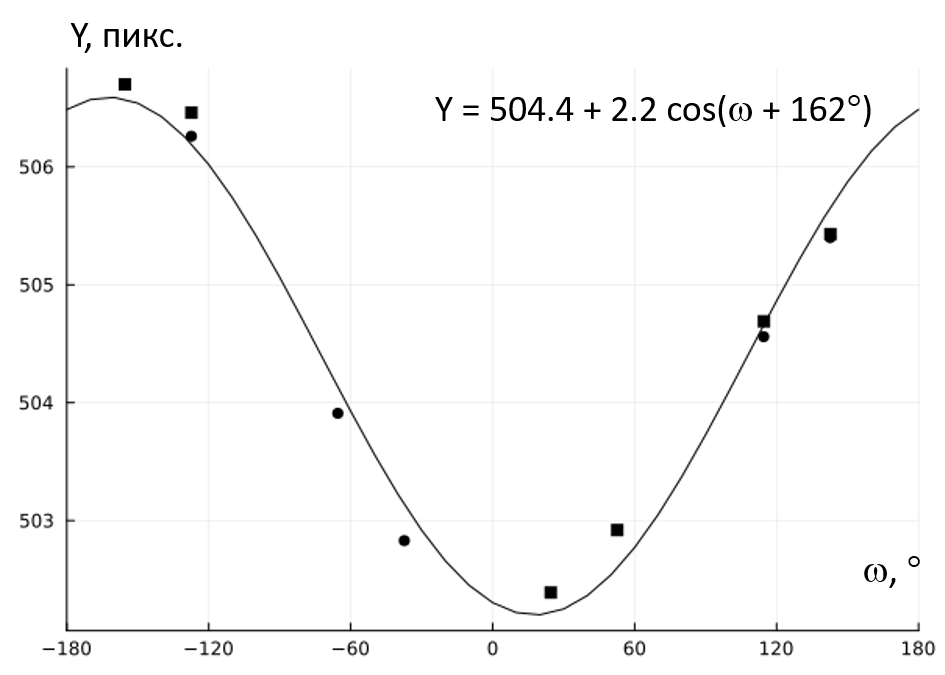
\includegraphics[width=0.8\textwidth]{eccentrGe.png}
    \caption{Зависимость координаты $Y$ от угла $\omega$ для монокристалла Ge. Для отрицательных (темные маркеры) и положительных (светлые маркеры) значениях $2\theta$ от значений $\omega$ были отняты значения $\theta + 90\degree$, тем самым позволив одновременно обработать все рефлексы. Аппроксимация функцией $Y = a_0 + a_1 \cos(\omega - \omega_1)$ выполнена с помощью МНК.}
    \label{fig:eccentrGe}
\end{figure}

\newpage
\bibliographystyle{unsrt}
\bibliography{bibliography}
\newpage
\section*{Приложение}
\begin{table}[ht!]
    \centering
    \begin{tabular}{ |c|c|c|c|c|c|c| }
        \hline
                    $hkl$ &           $D,\unit{мм}$ &  $2\theta_D, \ \degree$ &     $\varphi, \ \degree$ & $\omega, \ \degree$ &    $Y,\unit{пикс.}$ &    $X,\unit{пикс.}$ \\
        \hline
        $  \hkl(11 -1 3)$ & \multirow{20}{*}{128.5} & \multirow{10}{*}{-96.7} &  \multirow{2}{*}{-66.31} &                88.2 &              504.77 &              389.27 \\
        $ \hkl(-11 1 -3)$ &                         &                         &                          &               -91.8 &              503.78 &              389.53 \\
        $   \hkl(5 9 -5)$ &                         &                         &   \multirow{2}{*}{28.72} &                84.7 &              505.36 &              389.40 \\
        $  \hkl(-5 -9 5)$ &                         &                         &                          &               -95.3 &              503.24 &              389.41 \\
        $  \hkl(5 -9 -5)$ &                         &                         &  \multirow{2}{*}{119.20} &               -99.5 &              501.71 &              389.28 \\
        $   \hkl(-5 9 5)$ &                         &                         &                          &                80.5 &              506.90 &              389.58 \\
        $   \hkl(3 1 11)$ &                         &                         & \multirow{2}{*}{-138.01} &                97.4 &              505.92 &              389.33 \\
        $\hkl(-3 -1 -11)$ &                         &                         &                          &               -82.6 &              502.68 &              389.32 \\
        $  \hkl(3 -1 11)$ &                         &                         & \multirow{2}{*}{-143.63} &                84.6 &              505.92 &              389.35 \\
        $ \hkl(-3 1 -11)$ &                         &                         &                          &               -95.4 &              502.63 &              389.29 \\
        $ \hkl(1 -3 -11)$ &                         &  \multirow{10}{*}{96.7} &  \multirow{2}{*}{-59.35} &               -89.3 &              505.08 &              388.48 \\
        $  \hkl(-1 3 11)$ &                         &                         &                          &                90.7 &              504.09 &              388.18 \\
        $   \hkl(9 -1 7)$ &                         &                         &   \multirow{2}{*}{14.46} &                83.3 &              502.92 &              388.53 \\
        $  \hkl(-9 1 -7)$ &                         &                         &                          &               -96.7 &              506.04 &              388.01 \\
        $   \hkl(9 5 -5)$ &                         &                         &  \multirow{2}{*}{121.79} &                99.7 &              503.80 &              388.21 \\
        $  \hkl(-9 -5 5)$ &                         &                         &                          &               -80.3 &              505.05 &              388.27 \\
        $  \hkl(-3 11 1)$ &                         &                         & \multirow{2}{*}{-142.92} &                95.7 &              504.66 &              388.19 \\
        $ \hkl(3 -11 -1)$ &                         &                         &                          &               -84.4 &              504.08 &              388.26 \\
        \hline
    \end{tabular}
    \caption{Положения пиков $K\alpha_1$ для эталона Si.}
    \label{tab:Si}
\end{table}
\begin{table}[ht!]
    \centering
    \begin{tabular}{ |c|c|c|c|c|c|c| }
        \hline
                   $hkl$ &           $D,\unit{мм}$ &  $2\theta_D, \ \degree$ &     $\varphi, \ \degree$ & $\omega, \ \degree$ &    $Y,\unit{пикс.}$ &    $X,\unit{пикс.}$ \\
        \hline
        $ \hkl(-6 0 10)$ & \multirow{12}{*}{128.5} &  \multirow{6}{*}{-93.9} & \multirow{12}{*}{-179.06}&              -112.4 &              503.91 &              388.61 \\
        $ \hkl(6 0 -10)$ &                         &                         &                          &                67.6 &              504.56 &              388.47 \\
        $ \hkl(-10 0 6)$ &                         &                         &                          &               -84.3 &              502.83 &              388.50 \\
        $ \hkl(10 0 -6)$ &                         &                         &                          &                95.7 &              505.40 &              388.62 \\
        $  \hkl(6 0 10)$ &                         &                         &                          &              -174.3 &              506.26 &              388.64 \\
        $  \hkl(10 0 6)$ &                         &                         &                          &               157.6 &              506.70 &              388.74 \\
        $\hkl(-10 0 -6)$ &                         &  \multirow{6}{*}{93.9}  &                          &              -108.5 &              502.39 &              386.91 \\
        $  \hkl(10 0 6)$ &                         &                         &                          &                71.5 &              506.70 &              387.32 \\
        $\hkl(-6 0 -10)$ &                         &                         &                          &               -80.4 &              502.92 &              386.82 \\
        $  \hkl(6 0 10)$ &                         &                         &                          &                99.6 &              506.46 &              387.29 \\
        $ \hkl(10 0 -6)$ &                         &                         &                          &                 9.7 &              505.43 &              387.21 \\
        $ \hkl(6 0 -10)$ &                         &                         &                          &               -18.4 &              504.69 &              387.11 \\
        \hline
    \end{tabular}
    \caption{Положения пиков $K\alpha_1$ для эталона Ge.}
    \label{tab:Ge}
\end{table}
\end{document}
